\begin{figure}[htbp]
\centering
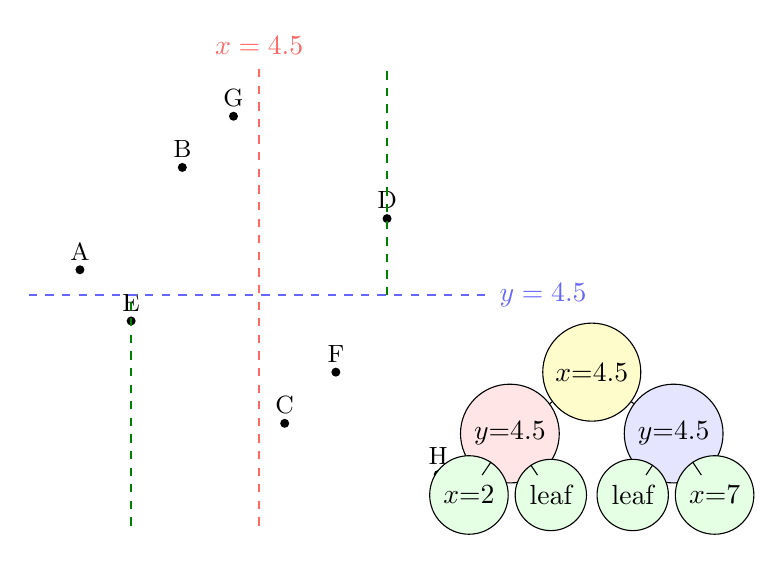
\begin{tikzpicture}[scale=0.65]
  \foreach \p/\l in {(1,5)/A, (3,7)/B, (5,2)/C, (7,6)/D, (2,4)/E, (6,3)/F, (4,8)/G, (8,1)/H} {
    \fill \p circle (2.5pt) node[above] {\small \l};
  }
  \draw[red!60,thick,dashed] (4.5,0)--(4.5,9) node[above] {$x=4.5$};
  \draw[blue!60,thick,dashed] (0,4.5)--(9,4.5) node[right] {$y=4.5$};
  \draw[green!50!black,thick,dashed] (2,0)--(2,4.5);
  \draw[green!50!black,thick,dashed] (7,4.5)--(7,9);
  \begin{scope}[xshift=11cm,yshift=3cm,scale=0.8]
    \node[draw,circle,fill=yellow!20] (root) at (0,0) {$x{=}4.5$};
    \node[draw,circle,fill=red!10] (l) at (-2,-1.5) {$y{=}4.5$};
    \node[draw,circle,fill=blue!10] (r) at (2,-1.5) {$y{=}4.5$};
    \node[draw,circle,fill=green!10] (ll) at (-3,-3) {$x{=}2$};
    \node[draw,circle,fill=green!10] (lr) at (-1,-3) {leaf};
    \node[draw,circle,fill=green!10] (rl) at (1,-3) {leaf};
    \node[draw,circle,fill=green!10] (rr) at (3,-3) {$x{=}7$};
    \draw (root)--(l) (root)--(r);
    \draw (l)--(ll) (l)--(lr);
    \draw (r)--(rl) (r)--(rr);
  \end{scope}
\end{tikzpicture}
\caption{KD-tree: (left) recursive axis-aligned partitioning of 2D space; (right) the corresponding binary tree structure.}
\label{fig:kd_tree}
\end{figure}
